\subsection{Breadth First Search}
\noindent Breadth-First Search (BFS) is an algorithm used for traversing or searching graph structures. It explores all neighbors of a node before moving to the next level, ensuring that it finds the shortest path in an unweighted graph. BFS operates using a queue, processing nodes in a first-in, first-out (FIFO) order. This guarantees that the shallowest (least depth) solution is found first, making it particularly useful in scenarios where all edges have equal cost.

\begin{figure}[H]
	\centering
	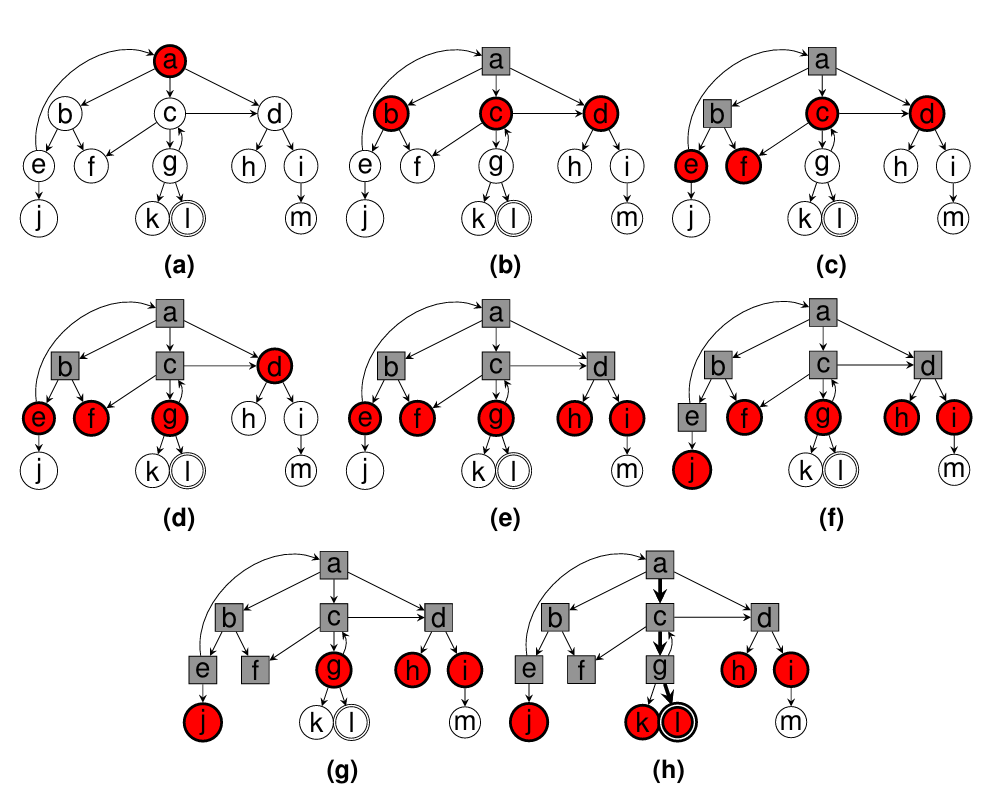
\includegraphics[width=0.8\textwidth]{./imgs/bfs.png}
	\caption{Breadth First Search (BFS)}
\end{figure}

\subsubsection{Pseudocode}
\begin{algorithm}[H]
	\caption{Breadth First Search (\textit{start, goal})}\label{alg:bfs}
	\begin{algorithmic}[1]
		\State queue \(gets\) [start]
		\While {queue is not empty}
		\State node \(gets\) dequeue(queue)
		\If {node = goal}
		\State return path
		\EndIf
		\ForAll {neighbor in valid moves}
		\If {neighbor not visited}
		\State mark neighbor as visited
		\State enqueue(queue, neighbor)
		\EndIf
		\EndFor
		\EndWhile
		\State return failure
	\end{algorithmic}
\end{algorithm}

\subsubsection{Implementation}
\begin{itemize}
	\item \textbf{\_\_init\_\_(\ldots)}
	      Initializes the BFS algorithm with grid dimensions, matrix representation, initial player position, stone positions, and switch positions. It also includes an optional deadlock detection flag.

	\item \textbf{search()}
	      Implements the BFS algorithm using a queue (FIFO). The search begins with the initial state in the frontier. The function explores states by dequeuing from the front, checking for the goal condition, and enqueuing valid new states.

	\item \textbf{can\_go(current\_state, dir)}
	      Checks whether the player can move in a given direction from the current state without encountering obstacles.

	\item \textbf{go(current\_state, dir)}
	      Generates a new state by moving the player in the specified direction, updating the relevant positions.

	\item \textbf{construct\_path(final\_state)}
	      Reconstructs the sequence of moves leading to the goal state by backtracking from the final state.

\end{itemize}


\subsubsection{Time and Space Complexity}
\textbf{Time Complexity:} \( O(b^d) \), where \( b \) is the branching factor and \( d \) is the depth of the shallowest solution. It explores all nodes at the current depth before moving deeper.

\textbf{Space Complexity:} \( O(b^d) \), as it stores all nodes at the current depth in memory.
